\section{The Safety Assessment Process}
\label{sec:process}
As the capabilities of technology grows, so does the complexity and capabilities of mechanical and electrical systems. Many of these systems are safety critical; the loss of correct functioning leads to loss of life, substantial material or environmental damage, or large monetary losses~\cite{SAE}. The development of such complex systems can benefit from a process with clearly defined design and implementation phases, and can further be subdivided into several sub-processes and phases. Analyses can be performed for each of the phases and when the analyses provide satisfactory outcomes, the process transitions into the next phase. 

In general, each field relies on various interpretations of the development process. In the field of aerospace technologies, the Aerospace Recommended Practice (ARP) documents are commonly referenced. The Society of Automotive Engineers (SAE) is an association of engineers and professionals devoted to the standards that guide the development of transportation systems~\cite{SAE:ARP4761, SAE:ARP4754A}. 

\begin{figure}[!htb]
        \center{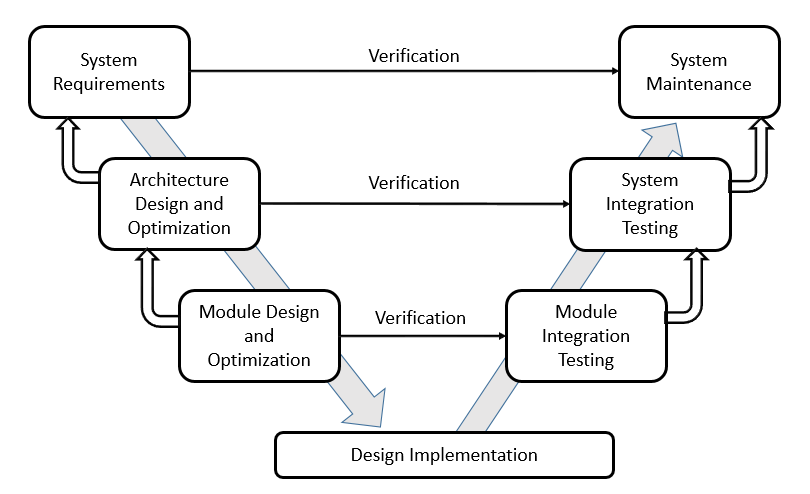
\includegraphics[width=0.85\textwidth] {images/v1.png}}
        \caption{\label{fig:v1} The V Model in System Development}
\end{figure}

The V model in software engineering, shown in Figure~\ref{fig:v1}, relates steps of the design phase with a post-implementation phase. It describes how the requirements are produced in the design phase and then how those requirements are verified against the implementation in the post-implementation phase. The left side of the V describes high-level design; the requirements of the system drive the design. The right side of the V describes the low-level implementation and testing of each module independently and as a whole. 

ARP4754A, the Guidelines for Development of Civil Aircraft and Systems~\cite{SAE:ARP4754A}, provides guidance on applying development assurance at each hierarchical level throughout the development life cycle of highly-integrated/complex aircraft systems. It has been recognized by the Federal Aviation Administration (FAA) as an acceptable method to establish the safety assurance process. The safety assessment process is a starting point at each hierarchical level of the development life cycle and is tightly coupled with the system development and verification processes. It is used to show compliance with certification requirements and for meeting a company's internal safety standards~\cite{SAE:ARP4754A} . 

\begin{figure}[!htb]
        \center{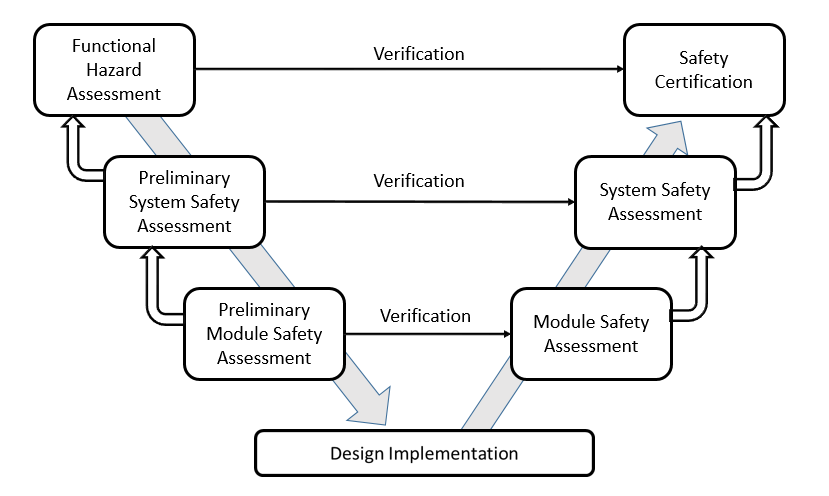
\includegraphics[width=0.85\textwidth] {images/v2.png}}
        \caption{\label{fig:v2} The V Model in Safety Assessment}
\end{figure}

The safety assessment shown in Figure~\ref{fig:v2} integrates each phase of the V model with analyses specific to system hazards and their severity. It also shows how these hazards should be addressed within the design phase. 
\begin{comment}
\danielle{Should I put these definitions in an appendix, leave them, or cut them entirely? The paragraphs following the description has the high level ideas...} The safety assessment process is defined in ARP4754A by the following phases:

\begin{description}
\item[Functional Hazard Assessment (FHA)] examines the functions of the system to identify potential functional failures and classifies the potential hazards associated with them. This includes identification of failure conditions, identifying the effects of those failures, classification of each failure condition, and assignment to safety objectives.

\item[Common Cause Analysis (CCA)] verifies and establishes physical and functional separation, isolation, and independence requirements between subsystems and verifies that these requirements have been met.

\item[Preliminary Aircraft Safety Assessment (PASA)] establishes aircraft safety requirements and provide a preliminary indication that the aircraft can meet those safety requirements.

\item[Preliminary System Safety Assessment (PSSA)] examines the proposed architecture(s) to determine how failures could cause the failure conditions determined by the FHA. The objective is to complete the safety requirements of an aircraft or system and show that the proposed system architecture satisfies the safety requirements. The PSSA is an iterative process that is performed at multiple stages of system development. 

\item[Fault Tree Analysis (FTA)] is performed to find combinations of faults that lead to the violation of a safety requirement. The fault tree itself shows the logical relation between the sets of faults and the violation of a safety requirement.

\item[Common Mode Analysis (CMA)] analyzes designs and implementations for elements that may defeat the redundancy
or independence of functions within the design, i.e. if elements are shown as independent in FTA, make sure they are truly independent in the system under consideration.

\item[Failure Modes and Effect Analysis (FMEA)] aims at finding the causality relationship between sets of faults, intermediate events, and undesired states in the system. Usually this is represented in tabular form and called an \textit{FMEA table}.

\item[Aircraft Safety Assessment (ASA)/System Safety Assessment (SSA)] verifies that the system (or aircraft), as implemented, meets the safety requirements specified by the PSSA.

\end{description}
\end{comment}

The safety assessment process includes safety requirements identification (left side of V) and verification (right side of V) supporting the aircraft development activities. The aircraft-level Functional Hazard Analysis (FHA) is conducted at the beginning of the development cycle and is followed by system level Functional Hazard Analysis for individual subsystems. The FHA is followed by the Preliminary System Safety Assessment (PSSA), which derives safety requirements for the subsystems, primarily using Fault Tree Analysis (see Section 2.1.1 for more information on fault trees). The PSSA process iterates throughout the design evolution as potential safety problems are identified and addressed through design changes. Once design and implementation are completed, the System Safety Assessment (SSA) process verifies whether the safety requirements are met in the implemented design. 

Both the preliminary safety assessment and the system safety assessment relies on safety related artifacts that describe the behavior of the system in the presence of faults. These artifacts are used throughout the entire process of development and are ubiquitous in the field of safety analysis. The most important of these for this research are fault trees and minimal cut sets. 







\begin{comment}
\subsection{Proposed Model Based Safety Assessment Process Supported by Formal Methods}
We propose a model-based safety assessment process backed by formal methods to help safety engineers with early detection of the design issues.  This process uses a single unified model to support both system design and safety analysis; this is shown in Figure~\ref{fig:SACycle1} and is based on the following steps:

\begin{enumerate}
	\item System engineers capture the critical information in a shared model:  high-level hardware and software architecture, nominal behavior at the component level, and safety requirements at the system level.
	\item System engineers use a model checker to check that the safety requirements are satisfied by the nominal design model. 
	\item Safety engineers augment the nominal model with the component failure modes. In addition, safety engineers specify the fault hypothesis for the analysis which corresponds to how many simultaneous faults the system must be able to tolerate.
	\item Safety engineers use a model checker to analyze if the safety requirements and fault tolerance objectives are satisfied by the design in the presence of faults. If the design does not tolerate the specified number of faults (or probability threshold of fault occurrence), then the tool produces counterexamples or minimal sets of fault combinations that can cause the safety requirement to be violated.
	\item The safety engineers examine the results to assess the validity of the fault combinations and the fault tolerance level of the system design. If a design change is warranted, the model will be updated with the latest design change and the above process is repeated.
\end{enumerate}

\begin{figure}[h]
	\begin{center}
		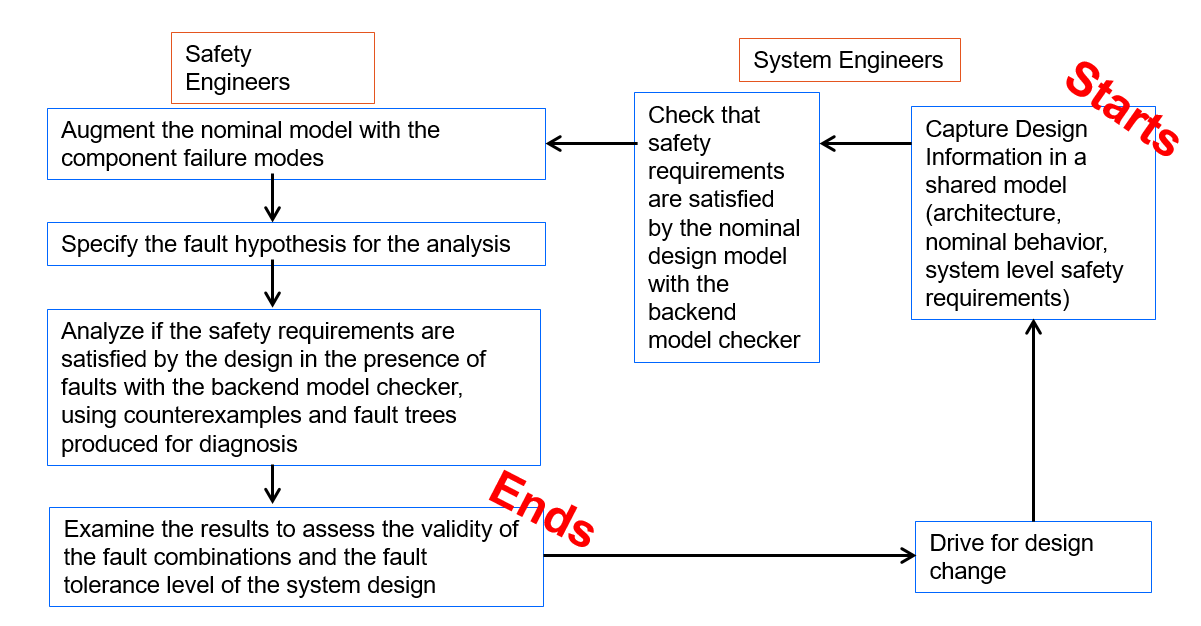
\includegraphics[width=\textwidth]{images/SACycle.PNG}
	\end{center}
	\caption{Proposed Steps of the Safety Assessment Process}
	\label{fig:SACycle1}
\end{figure}

These steps can be viewed as a cyclical process that involves both the system development engineers and the safety engineers of the system. Figure~\ref{fig:SACycle1} shows these steps within the context of the start and end of a project. 

\danielle{Add a bit more information here - pull from the MBSE project for IRAD. Include reasons why this approach is better, how it will help safety analysts, how it benefits the field as a whole. Then lead into the next sections with a statement about model checking, verification, etc.}
\end{comment}